
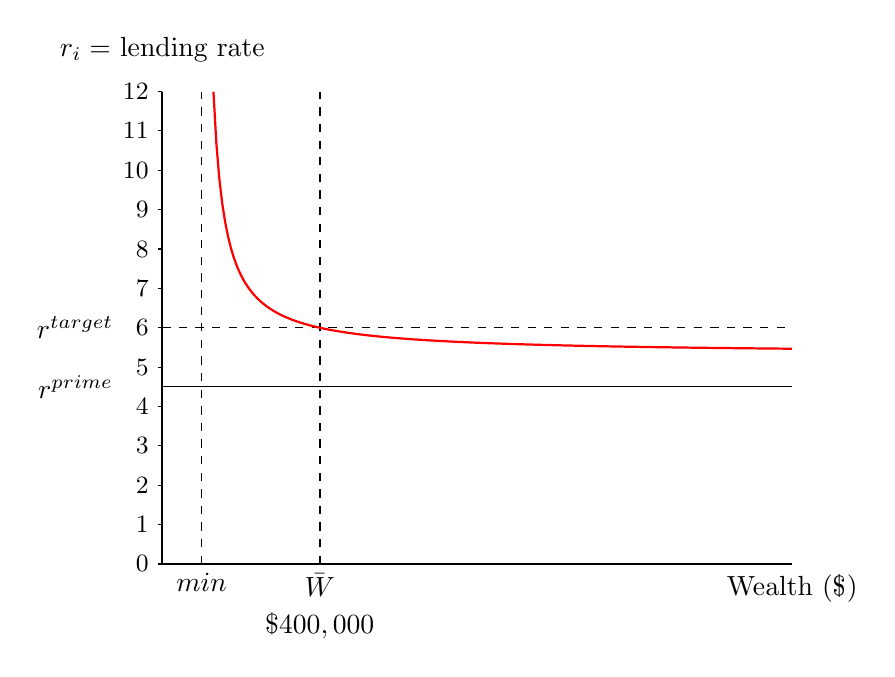
\begin{tikzpicture}[scale=.5].  %  Individual borrowing rate r\_i
%\def\bndmax{5}        %https://tex.stackexchange.com/questions/68462/filling-a-complex-region-with-tikz
%\def\bndmin{0.2}

\def \k {2}    % budget for rectangular hyperbola
\def \Wbar {4} % meam wealth in hundred thousands
\def \Wmin {1} % This sets the lower limit for lending in hundred thousands
\def \W {16}    % length  of x axis
\def \rbar {4.5} % N.B.:  this is r bar
\def \Y {12}     % height of y axis percent
\def \margin {1.5}
\def \target {\margin+\rbar} % target interest rate for bank
\def\bndmin {0.3} % This limits the function on the right so that it stays in the plotting frame
%\def \Wmin{(\B*\Wbar)/(\Y/\rbar-\A)} %function to keep in in bounds. NEEDS WORK
	
\tikzset{func/.style={thick}}	
\draw [thick] (0,\Y)node[above=.25cm]{$r_i=$ lending rate} -- (0,0)--(\W,0)node[below]{Wealth (\$)}node[below=.5cm] {};   	% Axes

\draw [thin] (0,\rbar) node[left=.5cm]{$r^{prime}$} -- (\W, \rbar);  	% % bank rate line
\draw [thin, dashed] (0,\target) node[left=.5cm]{$r^{target}$} -- (\W, \target);  	% % target rate line
\node at ( \Wbar, 0)[below=.5cm]{$\$400,000$};  
\foreach \yi in {0,...,\Y} \draw (0,\yi)--(-.1,\yi)node[left]{\small$\yi$};  %$ put the scale on the y axis

\draw [thick, dashed] (\Wbar, 0)node[below] {$\bar{W}$} --  (\Wbar, \Y);  	%. Wbar
\draw [thin, dashed]  (\Wmin, 0)node[below] {$min$} -- (\Wmin, \Y);  %minimum lending wealth

\draw[func,domain={\W-\Wmin}:\bndmin, red] plot [samples=200] (\x+\Wmin,{\target+\k/\x - \k/(\Wbar-\Wmin)});

\end{tikzpicture}


% \begin{tikzpicture}[scale=.5]
% %\def\bndmax{5}        %https://tex.stackexchange.com/questions/68462/filling-a-complex-region-with-tikz
% %\def\bndmin{0.2}
% \def \Y {10}  % height of y axis pecent
% \def \W {20}  % length  of x axis
% \def \Wbar {4} % jmeam wealth
% \def \omega {3} % N.B.:  this is r bar

% %Equation   \[ r_i = (A + .5 \frac{\bar{W}}{W_i})\omega\]
% \def \Wmin{.63}  %This sets the lower limit fo the 
% \def \Wmin{(\B*\Wbar)/(\Y/\omega-\A)} %function to keep in in bounds
	
% \tikzset{func/.style={thick}}	

% \draw [thick] (0,\Y)node[left=.5cm]{$r_i$} -- (0,0)--(\W,0)node[below]{Wealth};  	% Axes
% \draw [thick] (0,\omega)node[left=.5cm]{$\bar r$} -- (\W,\omega);  	% Axes
% \draw [thick,dashed] ( \Wbar,0)node[below=.5cm]{$\bar{W}$} -- (\Wbar,\Y);  	% Axes

% \foreach \yi in {0,...,\Y} \draw (0,\yi)--(-.1,\yi)node[left]{\small$\yi$};

% %     ORANGE
% % \def \A {1} \def \B {.8}
% % \draw[func,domain=\Wmin:\W, orange] plot [samples=200] (\x,{(\A/\x+\B*\X/\Wbar/\x)*\omega});
% % \def \A {1} \def \B {.1}
% % \draw[func,domain=\Wmin:\W, orange, dashed] plot [samples=200] (\x,{(\A+\B*\X/\Wbar/\x)*\omega});

% %     RED
% \def \A {1} \def \B {.8}
% \draw[func,domain=\Wmin:\W, red] plot [samples=200] (\x,{(\A+\B*\Wbar/\x)*\omega});
% \def \A {1} \def \B {.1}
% \draw[func,domain=\Wmin:\W, red, dashed] plot [samples=200] (\x,{(\A+\B*\Wbar/\x)*\omega});

% %.    BLUE
% \def \A {1} \def \B {.5}
% \draw[func,domain=\Wmin:\W, blue!90] plot [samples=200] (\x,{(\A+\B*\Wbar/\x)*\omega});
% %     GREEN
% \def \A {.8} \def \B {.8}
% \draw[func,domain=\Wmin:\W, green] plot [samples=200] (\x,{(\A+\B*\Wbar/\x)*\omega});
% %.    BLACK
% \def \A {.5} \def \B {.5}
% \draw[func,domain=\Wmin:\W, black] plot [samples=200] (\x,{(\A+\B*\Wbar/\x)*\omega});


% \draw [red,  thick](13, 9)--(15,9)node [right, black] {\small A=\ 1,\ B=0.8};
% \draw [red,  thick, dashed](13, 9.7)--(15,9.7)node [right, black] {\small A=\ 1,\ B=0.1};
% \draw [blue,  thick](13, 8.3)--(15,8.3)node [right, black] {\small A=\ 1,\ B=0.5};
% \draw [green, thick](13, 7.6)--(15,7.6)node [right, black] {\small A=.8, B=0.8};
% \draw [black, thick](13, 6.9)--(15,6.9)node [right, black] {\small A=.5, B=0.5};
% \end{tikzpicture}


